\section{Experimental Design}\label{sec:methodology}
In this section, we outline the methodology used in this study to address the challenges identified in Section~\ref{sec:problem_definition}. Our objective was to identify the most promising machine learning models and preprocessing techniques proposed from the literature, as outlined in Section~\ref{sec:related-work}, for predicting major oxide compositions from \gls{libs} data.
Then, using this knowledge, develop a pipeline that utilizes the strengths of these models and preprocessing techniques to improve prediction accuracy and robustness of the predictions.
We first describe the datasets used, including their preparation and the method of splitting for model training. Next, we outline the preprocessing steps and the model selection process, followed by a detailed explanation of the experimental setup and evaluation metrics. Finally, we discuss our validation testing procedures and the approach taken to ensure unbiased final model evaluations.


\subsection{Data Preparation}
Similarly to our previous work \citet{p9_paper}, we used the publicly available \gls{ccs} data from NASA's \gls{pds}~\cite{PDSGeoscienceNode}.
\gls{ccs} refers to \gls{libs} data that has been through a series of preprocessing steps such as subtracting the ambient light background, noise removal and removing the electron continuum to derive data that is more suitable for quantitative analysis.
A comprehensive description of this preprocessing procedure is available in \citet{wiensPreflightCalibrationInitial2013}.

\begin{table*}[h]
\centering
\begin{tabular}{llllllll}
\toprule
     wave &         shot1 &         shot2 &  $\cdots$ &        shot49 &       shot50  & median        & mean          \\
\midrule
240.81100 & 6.4026649e+15 & 4.0429349e+15 & $\cdots$  & 1.7922483e+15 & 1.7126615e+15 & 1.9892956e+15 & 1.7561699e+15 \\
240.86501 & 3.8557462e+12 & 2.2923680e+12 & $\cdots$  & 1.1355429e+12 & 8.6930379e+11 & 7.8172542e+11 & 7.2805052e+11 \\
$\vdots$  & $\vdots$      & $\vdots$      & $\cdots$  & $\vdots$      & $\vdots$      & $\vdots$      & $\vdots$      \\
905.38062 & 1.8823427e+08 & 58500403.     & $\cdots$  & -8449286.6    & 8710775.0     & 4.0513312e+09 & 5.2188327e+09 \\
905.57349 & 1.9864713e+10 & 1.2956832e+10 & $\cdots$  & 1.9785415e+10 & 7.1994239e+09 & 1.1311150e+10 & 1.2201224e+10 \\
\bottomrule
\end{tabular}
\caption{Example of CCS data for a single location (from \citet{p9_paper})}
\label{tab:ccs_data_example}
\end{table*}

While the \gls{ccs} data is in a more suitable form for quantitative analysis, it still requires further preprocessing. Table~\ref{tab:ccs_data_example} shows an example of the \gls{ccs} data for a single location of a sample. This corresponds to shots ($s$) and wavelength ($\lambda$) of the Intensity Tensor \ref{matrix:intensity} for this location.
The initial five shots from each sample are excluded because they are usually contaminated by dust covering the sample, which is cleared away by the shock waves produced by the laser \cite{cleggRecalibrationMarsScience2017}.
The remaining 45 shots from each location are then averaged, yielding a single spectrum $s$ per location $l$ in the Averaged Intensity Tensor\ref{matrix:averaged_intensity}, resulting in a total of five spectra for each sample. 

At this stage, the data still contains noise at the edges of the spectrometers.
These edges correspond to the boundaries of the three spectrometers, which collectively cover the \gls{uv}, \gls{vio}, and \gls{vnir} light spectra.
The noisy edge ranges are as follows: 240.811-246.635 nm, 338.457-340.797 nm, 382.138-387.859 nm, 473.184-492.427 nm, and 849-905.574 nm.
In addition to being noisy regions, these regions do not contain any useful information related to each of the major oxides.
Consequently, these regions are masked by zeroing out the values, rather than removing them, as they represent meaningful variation in the data~\cite{cleggRecalibrationMarsScience2017}.

Additionally, as a result of the aforementioned preprocessing applied to the raw \gls{libs} data, negative values are present in the \gls{ccs} data.
These negative values are not physically meaningful, since you cannot have negative light intensity \cite{p9_paper}.
Similar to the noisy edges, these negative values are also masked by zeroing out the values.

We transpose the data so that each row represents a location and each column represents a wavelength feature. 
Each location is now represented as a vector of wavelengths, with the corresponding average intensity values for each wavelength. 
These vectors are then concatenated to form a tensor, giving us the full Averaged Intensity Tensor.

For each sample, we have a corresponding set of major oxide compositions in weight percentage (wt\%).
These compositions are used as the target labels for the machine learning models.
An excerpt of this data is shown in Table \ref{tab:composition_data_example}.
While the \textit{Target}, \textit{Spectrum Name}, and \textit{Sample Names} are part of the dataset, our analysis focuses primarily on the \textit{Sample Names}.
The concentrations of the eight oxides \ce{SiO2}, \ce{TiO2}, \ce{Al2O3}, \ce{FeO_T}, \ce{MnO}, \ce{MgO}, \ce{CaO}, \ce{Na2O}, and \ce{K2O} represent the expected values for these oxides in the sample, serving as our ground truth. The \textit{MOC total} is not utilized in this study.

\begin{table*}[h]
\centering
\begin{tabular}{lllllllllllll}
\toprule
     Target & Spectrum Name & Sample Name & \ce{SiO2} & \ce{TiO2} & \ce{Al2O3} & \ce{FeO_T} & \ce{MnO} & \ce{MgO} & \ce{CaO} & \ce{Na2O} & \ce{K2O} & \ce{MOC total} \\
\midrule
AGV2 & AGV2 & AGV2 & 59.3 & 1.05 & 16.91 & 6.02 & 0.099 & 1.79 & 5.2 & 4.19 & 2.88 & 97.44 \\
BCR-2 & BCR2 & BCR2 & 54.1 & 2.26 & 13.5 & 12.42 & 0.2 & 3.59 & 7.12 & 3.16 & 1.79 & 98.14 \\
$\vdots$ & $\vdots$ & $\vdots$ & $\vdots$ & $\vdots$ & $\vdots$ & $\vdots$ & $\vdots$ & $\vdots$ & $\vdots$ & $\vdots$ & $\vdots$ & $\vdots$ \\
TB & --- & --- & 60.23 & 0.93 & 20.64 & 11.6387 & 0.052 & 1.93 & 0.000031 & 1.32 & 3.87 & 100.610731 \\
    TB2 & --- & --- & 60.4 & 0.93 & 20.5 & 11.6536 & 0.047 & 1.86 & 0.2 & 1.29 & 3.86 & 100.7406 \\
\bottomrule
\end{tabular}
\caption{Excerpt from the composition dataset (from \citet{p9_paper})}
\label{tab:composition_data_example}
\end{table*}

The major oxide weight percentages are appended to the matrix of spectral data, forming the final dataset.
This dataset is shown in Table~\ref{tab:final_dataset_example}.
The \textit{Target} column corresponds to the sample name, while the \textit{ID} column contains the unique identifier for each location.

\begin{table*}[h]
\centering
\footnotesize
\begin{tabular}{llllllllllllllllllllll}
\toprule
    240.81   & $\cdots$     & 425.82    & 425.87   & $\cdots$ & 905.57  & \ce{SiO2} & \ce{TiO2} & \ce{Al2O3} & \ce{FeO_T} & \ce{MgO} & \ce{CaO} & \ce{Na2O} & \ce{K2O} & Target     & ID \\
\midrule
	0        & $\cdots$     & 1.53e+10 & 1.62e+10 & $\cdots$ & 0        & 56.13     & 0.69 & 17.69 & 5.86 & 3.85 & 7.07 & 3.32 & 1.44 & jsc1421     & jsc1421\_2013\_09\_12\_211002\_ccs \\
	0        & $\cdots$     & 1.28e+10 & 1.30e+10 & $\cdots$ & 0        & 56.13     & 0.69 & 17.69 & 5.86 & 3.85 & 7.07 & 3.32 & 1.44 & jsc1421     & jsc1421\_2013\_09\_12\_211143\_ccs \\
    0        & $\cdots$     & 1.87e+10 & 1.83e+10 & $\cdots$ & 0        & 56.13     & 0.69 & 17.69 & 5.86 & 3.85 & 7.07 & 3.32 & 1.44 & jsc1421     & jsc1421\_2013\_09\_12\_210628\_ccs \\
    0        & $\cdots$     & 1.77e+10 & 1.78e+10 & $\cdots$ & 0        & 56.13     & 0.69 & 17.69 & 5.86 & 3.85 & 7.07 & 3.32 & 1.44 & jsc1421     & jsc1421\_2013\_09\_12\_210415\_ccs \\
    0        & $\cdots$     & 1.75e+10 & 1.79e+10 & $\cdots$ & 0        & 56.13     & 0.69 & 17.69 & 5.86 & 3.85 & 7.07 & 3.32 & 1.44 & jsc1421     & jsc1421\_2013\_09\_12\_210811\_ccs \\
    0        & $\cdots$     & 5.52e+10 & 3.74e+10 & $\cdots$ & 0        & 57.60     & 0.78 & 26.60 & 2.73 & 0.70 & 0.01 & 0.38 & 7.10 & pg7         & pg7\_2013\_11\_07\_161903\_ccs \\
    0        & $\cdots$     & 5.09e+10 & 3.41e+10 & $\cdots$ & 0        & 57.60     & 0.78 & 26.60 & 2.73 & 0.70 & 0.01 & 0.38 & 7.10 & pg7         & pg7\_2013\_11\_07\_162038\_ccs \\
    0        & $\cdots$     & 5.99e+10 & 3.97e+10 & $\cdots$ & 0        & 57.60     & 0.78 & 26.60 & 2.73 & 0.70 & 0.01 & 0.38 & 7.10 & pg7         & pg7\_2013\_11\_07\_161422\_ccs \\
    0        & $\cdots$     & 5.22e+10 & 3.47e+10 & $\cdots$ & 0        & 57.60     & 0.78 & 26.60 & 2.73 & 0.70 & 0.01 & 0.38 & 7.10 & pg7         & pg7\_2013\_11\_07\_161735\_ccs \\
    0        & $\cdots$     & 5.29e+10 & 3.62e+10 & $\cdots$ & 0        & 57.60     & 0.78 & 26.60 & 2.73 & 0.70 & 0.01 & 0.38 & 7.10 & pg7         & pg7\_2013\_11\_07\_161552\_ccs \\
	$\vdots$ & $\cdots$ & $\vdots$ & $\vdots$ & $\cdots$ & $\vdots$ & $\vdots$ & $\vdots$ & $\vdots$ & $\vdots$ & $\vdots$ & $\vdots$ & $\vdots$ & $\vdots$ & $\vdots$ & $\vdots$ \\
\midrule
\end{tabular}
\caption{Excerpt from the final dataset (values have been rounded to two decimal places for brevity).}
\label{tab:final_dataset_example}
\end{table*}


\subsection{Model and Preprocessing Selection}
For the initial investigative experiments, we selected a range of models for further exploration, namely \gls{svr}, \gls{gbr}, \gls{pls}, \gls{xgboost}, \gls{ngboost}, \gls{etr}, \gls{enet}, and \gls{sgdr}.
We also included regular \gls{ann} and \gls{cnn} in this phase of experimentation.
This selection was guided primarily by the literature review but also by exploratory intuition, aiming to discover potentially innovative applications and performances within our specific dataset.

Our literature review highlighted various approaches and their effectiveness in handling the challenges associated with predicting major oxide compositions from \gls{libs} data.
For instance, \citet{andersonImprovedAccuracyQuantitative2017} discussed the use of multiple regression models, finding that different models excelled with specific oxides, which informed our model-specific approach.
\citet{song_DF-K-ELM} presented a hybrid model combining domain knowledge with machine learning, which inspired our interest in models that could offer both high performance and interpretability. \citet{rezaei_dimensionality_reduction} demonstrated the beneficial impact of dimensionality reduction techniques like \gls{pca}, which we considered essential for managing our high-dimensional \gls{libs} data.

All models were evaluated for their performance across each of the major oxides relevant to this study. 
Our preliminary analysis indicated model-specific strengths, suggesting the potential for leveraging different models for specific prediction tasks. 
This observation motivated us to develop architectural frameworks designed to systematically capitalize on the strengths of each model for specific oxides

An interesting discovery from our literature review was a study on the stacking and chaining of normalization methods initially aimed at classification contexts.
Inspired by these ideas, we explored the possibility of improving model performance by optimizing the preprocessing chain for each model, per oxide, in order to determine which normalization methods would be most beneficial.
For this purpose, we considered the following preprocessing techniques: Min-Max normalization, Z-Score normalization, Robust Scaling, Max Absolute Scaling, Norm 3, Quantile Transformer and Power Transformer.
Additionally, we also considered dimensionality reduction techniques such as \gls{pca} and \gls{kernel-pca}.
Through experimentation, we identified which preprocessing techniques were most effective for each model and oxide.
Realizing the potential of this, we decided to further investigate how the predictive accuracy and robustness could be improved by combining the strengths of these models and preprocessing techniques.
From our investigation, we determined that the stacking ensemble method seemed very promising and novel in the LIBS analysis field, leading us to select it as the primary method for our study.

Stacking ensemble is analogous to the methodologies employed in the original \gls{moc} pipeline, which also tailored predictions for each oxide by blending outputs from the \gls{pls1-sm} and \gls{ica} phases, variably weighting the influence of the \gls{ica} predictions depending on the oxide.
Unlike the \gls{moc} model, which required manual determination of the model weightings for each oxide, our method utilizes a meta learner to learn optimal parameter settings.
Stacking ensemble is beneficial as it dynamically adapts to our dataset's characteristics without the need for domain-specific knowledge.
This approach represents a more sophisticated method, streamlining complex model configurations and potentially enhancing predictive accuracy through dynamically learned integrations, rather than fixed presets.


\subsection{Experimental Setup}
Experiments were conducted on a machine equipped with an Intel Xeon Gold 6242 CPU, featuring 16 cores and 32 threads.
The CPU has a base clock speed of 2.80 GHz and a maximum turbo frequency of 3.90 GHz.
The system has 64 GB of RAM and runs on Ubuntu 22.04.2 LTS.
Models were implemented using Python 3.10.11.
The primary libraries used were Scikit-learn 1.4.2, XGBoost 2.0.3, Torch 2.2.2, NumPy 1.26.4, Pandas 2.2.1, Keras 3.2.1 and Optuna 3.6.1.

% \subsection{Validation and Testing Procedures}
\subsection{Validation and Testing Procedures for Model Evaluation}\label{subsec:validation_testing_procedures}
This section describes the validation and testing procedures our experiments follow.
Selecting appropriate testing procedures is crucial for ensuring the validity and reliability of the results.
For that reason, we delineate a methodological approach that ensures our models are accurate and generalizable.

We have chosen to test and evaluate all our experiments using both cross-validation and a separate test set.
Evaluating results solely on the test set could lead to models that are overly specialized to the test set.
This occurs when searching for the optimal configuration of hyperparameters specifically tailored to the test set.
However, our objective is to develop models that demonstrate high accuracy and robustness, even on entirely unseen data.
To achieve this, we employ k-fold cross-validation to ensure our models have high generalizability, thereby increasing the likelihood that they will perform as expected on new data.

We use an $80\%/20\%$ split for training and testing sets. The training set is further subdivided into $4$ folds, which are used for cross validation.

While we employ conventional techniques like holdout sets and k-fold cross validation, the dataset we use imposes additional challenges to the process.

One of the primary challenges is preventing data leakage.
As per concentration matrix $\mathbf{C}$ in Section~\ref{sec:problem_definition}, each target only has one ground truth concentration value per oxide.
However, each target is shot at multiple locations, resulting in multiple instances of the same target in the dataset, as shown in Table~\ref{tab:final_dataset_example}.
Although the intensity values vary for each location, they fundamentally represent measurements of the same target.
If we were to randomly split the dataset, some locations from a target could end up in the testing set while others remain in the training set.
This would cause data leakage, as the testing set would no longer consist solely of unseen targets.
To prevent this, we ensure that each target is represented only once in the dataset by grouping data from all locations on a given target.

Furthermore, the limited availability of data, as mentioned in Section~\ref{sec:problem_definition}, poses another significant challenge due to the difficult collection process.
The dataset we use consists of 408 samples, which is relatively large by \gls{libs} standards.
However, there are only a few samples with concentration values for the oxides in the targets that are either very high or very low compared to the rest of the data, which we call extreme values.
These less frequent high and low concentration values can be problematic.
If such values end up in the test set, the model may be evaluated on data points outside the range it was trained on.
This situation can lead to an inaccurate assessment of the model's performance, as it might not handle these less common concentration ranges effectively.

When performing a random split of the dataset into multiple folds for cross-validation, as well as for training and testing sets, this small number of extreme values can result in an uneven distribution.
The presence or absence of these extreme values in any given fold can heavily influence the model's performance metrics.
If extreme values are disproportionately allocated to the testing set, the resulting model may struggle to generalize accurately.
This uneven distribution can lead to models that perform well on the majority of the data but fail to predict accurately for these extreme concentration values, which are critical in many practical applications.
Conversely, if the scarce extreme values are disproportionately assigned to the training set, the model may become overly specialized in handling these extreme values, potentially leading to overfitting.
This means the model might perform well on the training set, including the extreme values, but fail to generalize effectively to new, unseen data, especially if the test set does not contain similar extreme values.
This could result in an inaccurate assessment of the model's performance, as the test set would not adequately challenge the model's ability to predict across the full range of data variability.

\begin{figure*}[h!]
    \centering
    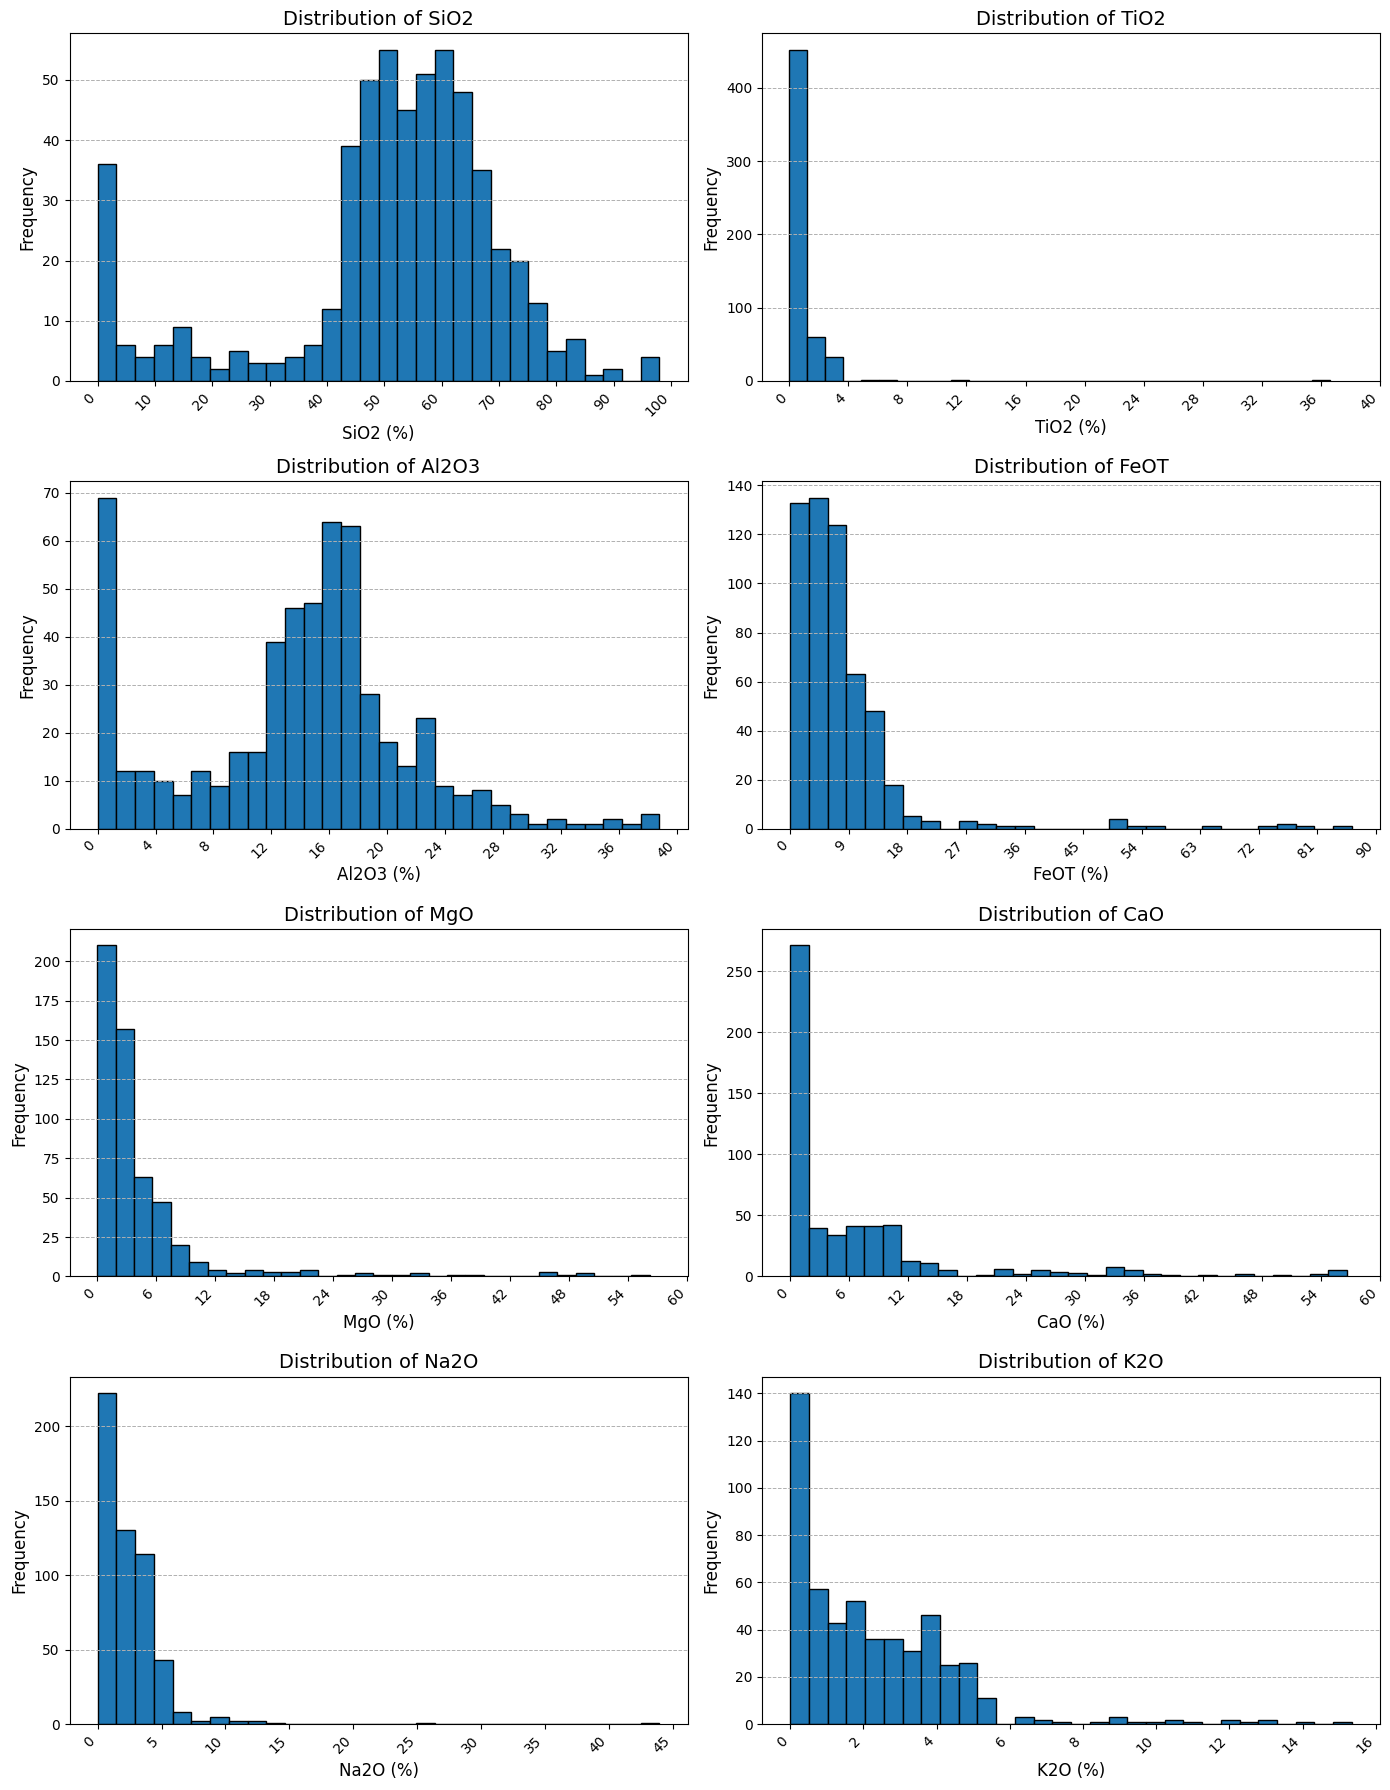
\includegraphics[width=\textwidth]{images/oxide_distributions.png}
    \caption{Distributions of various oxide concentrations in the dataset. The histograms show the frequency of concentration values for \ce{SiO2}, \ce{TiO2}, \ce{Al2O3}, \ce{FeO_T}, \ce{MgO}, \ce{CaO}, \ce{Na2O}, and \ce{K2O}.}
    \label{fig:oxide_distributions}
\end{figure*}

Figure~\ref{fig:oxide_distributions} illustrates the distributions of various oxide concentrations in our dataset.
Across all oxides, there is a general pattern of skewed distributions, with concentrations heavily weighted towards lower values.
This is particularly notable in \ce{TiO2}, \ce{FeO_T}, \ce{MgO}, \ce{CaO}, and \ce{Na2O}.
\ce{SiO2} and \ce{Al2O3} show more variability, with \ce{SiO2} exhibiting a bimodal distribution.
These distributions confirm the presence of extreme values across all oxides, which are significantly overrepresented or underrepresented, further complicating the model training process.

This necessitates careful dataset partitioning to ensure that the model training process accounts for these challenges, improving the generalizability and robustness of the models.

\subsubsection{Dataset Partitioning}\label{subsubsec:dataset_partitioning}
To ensure rigorous evaluation of our models and to address the challenges of data leakage and uneven distribution of extreme values, we have implemented a customized k-fold data partitioning procedure. 
This approach divides the dataset into $k$ folds, which it uses to define cross-validation data sets, as well as a training set and a test set.
The procedure ensures that all data points from a given target are only present in one of the $k$ folds, overcoming the challenge of data leakage we mention above.
Additionally, it ensures that extreme values are handled by redistributing them evenly across the training folds, preventing any single fold from being disproportionately influenced by these values.

\begin{algorithm}
\caption{Data Partitioning With Extreme Value Handling}
\label{alg:custom_kfold_cv}
\begin{algorithmic}[1]
\Require Dataset $\mathbf{D}$, group column $g$, target column $t$, number of splits $k$, percentile $p$, random seed $\textit{seed}$
\Ensure Training and validation sets for cross-validation $\mathbf{T}_\text{cv}$, training set $\mathbf{D}_\text{train}$, and test set $\mathbf{D}_\text{test}$
\State \label{line:seed} Set random seed for reproducibility if $\text{seed}$ is not None
\State \label{line:remove_duplicates} Remove duplicate entries based on $g$ and sort by $t$
\State \label{line:assign_folds} Assign fold numbers sequentially from 0 to $k-1$ to unique targets
\If{extreme values handling is enabled}
    \State \label{line:identify_extremes} Identify extreme values at percentiles $p$ and $1-p$
    \State \label{line:reassign_extremes} Reassign extreme values to folds $0$ to $k-2$
\EndIf
\State \label{line:merge_folds} Merge fold assignments information into the original dataset
\State \label{line:split_dataset} Split dataset into test set $\mathbf{D}_\text{test}$ (fold $k-1$) and remaining data $\mathbf{D}_\text{train}$
\State \label{line:create_folds} Create $k-1$ training and validation sets
\For{each fold $i$ from 0 to $k-2$}
    \State $\mathbf{T}_\text{train}[i] \gets \mathbf{D}_\text{train} \setminus \text{fold}_i$
    \State $\mathbf{T}_\text{val}[i] \gets \text{fold}_i$
    \State Append $(\mathbf{T}_\text{train}[i], \mathbf{T}_\text{val}[i])$ to $\mathbf{T}_\text{cv}$
\EndFor
\State \label{line:remove_fold_column} Remove fold column from all datasets
\State \Return $\mathbf{T}_\text{cv}, \mathbf{D}_\text{train}, \mathbf{D}_\text{test}$
\end{algorithmic}
\end{algorithm}

The procedure outlined in Algorithm~\ref{alg:custom_kfold_cv} begins by setting a random seed for reproducibility if one is provided (Line~\ref{line:seed}).
This ensures that the results are consistent across different runs of the algorithm.
Next, the dataset is processed to remove any duplicate entries based on the group column $g$ and then sorted by the target column $t$ (Line~\ref{line:remove_duplicates}).
This step ensures that each group is uniquely identified and ordered appropriately.
The dataset we illustrate in Table~\ref{tab:final_dataset_example} would require a group column $g$ of "\texttt{Target}" to group the data by target.
The target column $t$ refers to the column with the target variable, which would be the oxide for which we are predicting the concentration, for example, \ce{SiO_2}.
By sorting the dataset by the target column $t$, we ensure that the data is ordered by the target concentration values in ascending order.

Fold numbers are then assigned sequentially using a modulo operation to ensure a random-like distribution of the unique targets across the folds (Line~\ref{line:assign_folds}).
This means that, while the assignment process follows a sequence, the resulting distribution of targets is effectively randomized.
Fold numbers start in 0 and go up to $k-1$, as implied by the modulo operation.
If handling of extreme values is enabled, the algorithm identifies the top and bottom percentiles of the target values (Line~\ref{line:identify_extremes}).
These extreme values are then reassigned to the training folds (0 to \( k-2 \)), ensuring they are evenly distributed across these folds (Line~\ref{line:reassign_extremes}).

The fold assignments are then merged into the original dataset, as described in Line~\ref{line:merge_folds}.
Essentially, this step enables the partitioning steps that follow, by ensuring each data item has an associated fold number.
Following this, the dataset is divided into a test set, which always consists of the data points assigned to fold $k-1$, and the remaining data forms the training set, as outlined in Line~\ref{line:split_dataset}.
The training data is further divided into $k-1$ sets for cross-validation. 
For each fold $i$ where $i \in \{0, 1, \ldots, k-2\}$, we create a cross-validation training set $\mathbf{T}_\text{train}[i]$ by excluding the $i$-th fold from the set of $k-1$ folds, and use the $i$-th fold as the validation set $\mathbf{T}_\text{val}[i]$.
These pairs of training and validation sets are then appended to the list of cross-validation sets $\mathbf{T}_\text{cv}$ (Line~\ref{line:create_folds}).

Finally, the fold indicator column is removed from all datasets before returning the final partitions (Line~\ref{line:remove_fold_column}).
The fold indicator column was added to keep track of which data points belong to which folds, which is crucial for ensuring that data points are correctly partitioned into their respective training and test sets during cross-validation. 
This cleanup step ensures that the fold information does not interfere with subsequent data processing or model training.

The final output of this procedure consists of:
\begin{itemize}
    \item A set of tuples \(\mathbf{T}_\text{cv}\), where each tuple contains a training set and a validation set.
    \item The overall training set \(\mathbf{D}_\text{train}\), consisting of all the data points not in the test set.
    \item The test set \(\mathbf{D}_\text{test}\), distinct from the training set.
\end{itemize}

The data partitioning does not modify the original dataset; it merely partitions it.
For that reason, each of the datasets that are returned has the same structure as shown in Table~\ref{tab:final_dataset_example}.

Our method for handling extreme values ensures that the test set does not include samples outside the range seen in the training set.
This approach addresses several critical challenges and represents a deliberate trade-off to improve the reliability of our model evaluation:

Firstly, it mitigates the risk of uneven distribution of extreme values, which can disproportionately affect model performance metrics.
If extreme values are unevenly distributed between the training and test sets, the evaluation of the model can be heavily skewed, leading to unreliable and misleading performance metrics.
By redistributing extreme values evenly across the training folds, we ensure a more balanced and fair assessment of the model's capabilities during cross-validation.

Secondly, this trade-off allows for a more stable and reliable assessment of the model's performance on typical data points.
While the test set may be less representative of the full range of data, particularly regarding rare extreme values, the evaluation focuses on the model's ability to generalize from the training data to new data within the same distribution range.
This is prudent because, in many practical applications, the reliability of the model on typical data points is more critical than its performance on rare extremes.
By using cross-validation in conjunction with a separate test set, we ensure that the model is robust and performs well under typical conditions.

However, it is important to recognize the limitation this approach introduces: excluding extreme values from the test set means we can only confidently assess the model's performance within the range of the test set.
If we receive predictions outside this range, we cannot reliably assert their accuracy, as the model has not been fully evaluated on such data.
This could potentially make the model less useful in scenarios where predictions on extreme values are critical.
Nevertheless, cross-validation partially mitigates this issue by allowing the model to learn from extreme values during the training and validation phases, thereby improving its robustness.
Metrics obtained from cross-validation provide a broader picture of the model's accuracy and robustness across the entire dataset, including extreme values.

Therefore, although our approach may make the test set less representative of the full dataset, it is a deliberate trade-off aimed at achieving a more accurate and reliable evaluation of the model's generalization performance.

Our method is inspired by the approach described by \citet{andersonImprovedAccuracyQuantitative2017}.
They employed a similar strategy to assess the performance of their PLS model, using k-fold cross-validation and a separate test set.
Their process involved dividing the full set of laboratory data into five folds, using four for cross-validation and combining them as the final training set, while the fifth fold served as a test set.
For consistency, we also use $k = 5$ for our data partitioning.
Given that the $k$-th fold is used as the test set, having $k=5$ results in 4 folds for cross-validation.

Additionally, by using $k = 5$ folds, we have effectively chosen an 80\%/20\% split between the training and testing datasets.
In our experience, this ratio maximizes the training set's capacity for effective model learning while ensuring that the testing set is sufficiently representative to provide an accurate assessment of the model's performance on new data.
Allocating too much data to the testing set could compromise the comprehensiveness of the training set, undermining the model's ability to generalize effectively due to the limited availability of data.

\subsubsection{Cross-Validation}
% Section on cross validation approach


\subsection{Summary}
